\documentclass{article}
\usepackage{xeCJK}
\usepackage{amsmath,esint,amssymb,amsthm}
\usepackage{hyperref}
\usepackage{tikz}
\usepackage[bottom]{footmisc}
\setCJKmainfont[AutoFakeBold]{SimSun}
\usepackage{bm}
\def\v#1{\overrightarrow{#1}}
\begin{document}
\title{笔记整理}
\author{赵丰}
\maketitle
\section{草稿}
涡量方程:
\eqref{eq:52NSEqUnCompress}式给出了不可压流的N-S方程,对于一般情形,在\eqref{eq:52TijUn}式中代入\eqref{eq:52TSG}式(取$\mu'=0$)于是有
\begin{align}
\nabla\cdot \bm{T} = & -\nabla p+\mu \nabla^2 \v{v} +\mu \frac{\partial^2 v_i}{\partial x_i \partial x_j} \v{e}_j + \frac{\partial }{\partial x_i} (-\frac{2}{3}\mu \nabla\cdot \v{v}\delta_{ij})\v{e}_j, \text{eq\eqref{eq:52nablav0C} invalid}\\
= & -\nabla p+\mu \nabla^2 \v{v} + \frac{\mu}{3}\nabla(\nabla \cdot \v{v})
\end{align}
因此我们得到一般形式的N-S方程:
\begin{equation}\label{eq:71generalNS}
\frac{\partial \v{v}}{\partial t}+\v{v}\cdot\nabla\v{v}=\v{f}-\frac{\nabla p}{\rho}+\frac{\mu}{\rho} (\frac{1}{3}\nabla(\nabla\cdot \v{v})+\nabla^2 \v{v})
\end{equation}

通过对上式两边取旋度可以得到涡量方程,为此,首先推导:
\begin{equation}\label{eq:71vvw}
2\v{v}\cdot \nabla \v{v}=\nabla (\v{v}\cdot\v{v}) + 2(\nabla\times \v{v})\times \v{v} 
\end{equation}

\begin{align*}
\text{RHS}=& \frac{\partial v_i^2}{\partial x_j} \v{e_j} + 2(\epsilon_{ijk}\frac{\partial v_k}{\partial x_j}\v{e_i})\times \v{v}\\
=& \frac{\partial v_i^2}{\partial x_j} \v{e_j} + 2(\epsilon_{min}\epsilon_{ijk}\frac{\partial v_k}{\partial x_j}v_n)\v{e_m}\\
=& 2v_i\frac{\partial v_i}{\partial x_j} \v{e_j} - 2((\delta_{mj}\delta_{nk}-\delta_{mk}\delta_{nj})\frac{\partial v_k}{\partial x_j}v_n)\v{e_m}\\
=& 2v_i\frac{\partial v_i}{\partial x_j} \v{e_j} - 2(\frac{\partial v_k}{\partial x_j}v_k)\v{e_j}+2(\frac{\partial v_k}{\partial x_j}v_j)\v{e_k}\\
=& 2(\frac{\partial v_k}{\partial x_j}v_j)\v{e_k}\\
= \text{LHS}
\end{align*}

再推导
\begin{equation}
\nabla\times(\v{A}\times \v{B})=(\nabla\cdot \v{B}+\v{B}\cdot\nabla)\v{A}-(\nabla\cdot \v{A}+\v{A}\cdot\nabla)\v{B}
\end{equation}

\begin{align*}
\text{LHS}=&\nabla\times(\epsilon_{ijk}A_jB_k\v{e_i})\\
=& \epsilon_{mni}\epsilon_{ijk}\frac{\partial (A_jB_k)}{\partial x_n}\v{e_m}\\
=& (\delta_{mj}\delta_{nk}-\delta_{mk}\delta_{nj})(B_k\frac{\partial A_j}{\partial x_n}+A_j\frac{\partial B_k}{\partial x_n})\v{e_m}\\
=&(B_k\frac{\partial A_j}{\partial x_k}+A_j\frac{\partial B_k}{\partial x_k})\v{e_j}
-(B_k\frac{\partial A_j}{\partial x_j}+A_j\frac{\partial B_k}{\partial x_j})\v{e_k}\\
=& \text{RHS}
\end{align*}

因此,由\eqref{eq:71generalNS}式我们有:
\begin{align*}
\nabla\times \text{LHS}=& \nabla\times (\frac{\partial \v{v}}{\partial t}+\v{v}\cdot\nabla\v{v})\\
=& \frac{\partial }{\partial t}(\nabla\times \v{v})+\nabla\times(\v{v}\cdot\nabla\v{v}) \\
=& \frac{\partial \v{w}}{\partial t}+\nabla\times(\nabla \frac{|\v{v}|^2}{2}+\v{w}\times \v{v})\\
=& \frac{\partial \v{w}}{\partial t} +(\nabla\cdot\v{v})\v{w}-(\nabla\cdot\v{w})\v{v}
+(\v{v}\cdot\nabla)\v{w}-(\v{w}\cdot\nabla)\v{v},\nabla\cdot\v{w}=0 \\
=& \frac{D \v{w}}{D t} +(\nabla \cdot \v{v})\v{w}-(\v{w}\cdot\nabla)\v{v}
\end{align*}

而上式右端:
\begin{align*}
\nabla\times \text{LHS}=& \nabla\times\left(\v{f}-\frac{\nabla p}{\rho}+\frac{\mu}{\rho} (\frac{1}{3}\nabla(\nabla\cdot \v{v})+\nabla^2 \v{v})\right)\\
=& \nabla\times \v{f}-\nabla\frac{1}{\rho}\times \nabla p + \frac{\mu}{\rho}\nabla\times \nabla^2\v{v}+\nabla\left(\frac{\mu}{\rho}\right)\times(\frac{1}{3}\nabla(\nabla\cdot \v{v})+\nabla^2 \v{v})
\end{align*}
因此我们由不可压的N-S方程得到了涡量方程的一般形式:
\begin{equation}
\frac{D \v{w}}{D t} +(\nabla \cdot \v{v})\v{w}-(\v{w}\cdot\nabla)\v{v}=\nabla\times \v{f}-\nabla\frac{1}{\rho}\times \nabla p + \frac{\mu}{\rho}\nabla\times \nabla^2\v{v}+\nabla\left(\frac{\mu}{\rho}\right)\times(\frac{1}{3}\nabla(\nabla\cdot \v{v})+\nabla^2 \v{v})
\end{equation}
从上面的涡量方程可以看出,对于理想正压流体,若质量力有势,方程右端项为零。
由连续性方程\eqref{eq:52ContiMaterial}式左端可化简为
\begin{equation}
\frac{1}{\rho}\frac{D\v{w}}{Dt}+\frac{D}{Dt}\left(\frac{1}{\rho}\right) \v{w}-\left(\frac{\v{w}}{\rho}\right)\cdot \nabla \v{v}=0
\end{equation}
即整理为
\begin{equation}
\frac{D}{Dt}\left(\frac{\v{w}}{\rho}\right)=\left(\frac{\v{w}}{\rho}\right)\cdot\nabla\v{v}
\end{equation}
%如何说明 Lagrange 定理??

% 下面以信风的形成为例说明非正压流场速度环量非零。

% \begin{figure}[!ht]
 % \centering
 % %LaTeX with PSTricks extensions
%%Creator: inkscape 0.92.2
%%Please note this file requires PSTricks extensions
%\documentclass{article}
%\pagestyle{empty}
%\usepackage{tikz}
%\begin{document}
 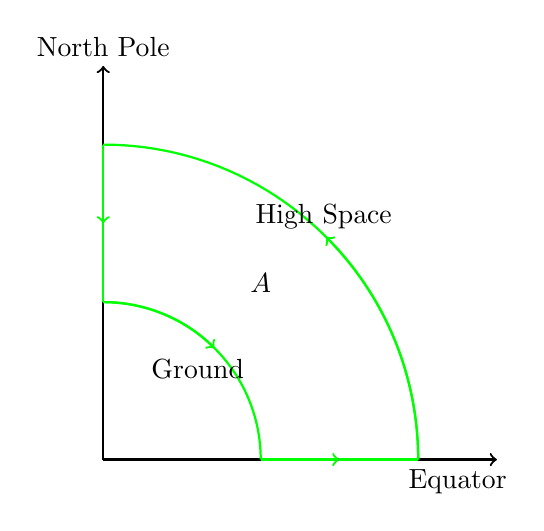
\begin{tikzpicture}
  \draw[thick,->] (0,0) -- (5,0);
  \draw[thick,->] (0,0) -- (0,5);
  \draw[thick,green,->] (2,0) -- (3,0);
  \draw[thick,green] (3,0) -- (4,0);  
  \draw[thick,green] (0,2) -- (0,3);
  \draw[thick,green,->] (0,4) -- (0,3);    
  \draw[thick,green] (2,0) arc [start angle=0, end angle=90, radius=2]; %ground
  \draw[thick,green,->] (0,2) arc [start angle=90, end angle=45, radius=2]; %ground
  \draw[thick,green] (4,0) arc [start angle=0, end angle=90, radius=4]; %high space
  \draw[thick,green,->] (4,0) arc [start angle=0, end angle=45, radius=4]; %high space
  \draw (4.5,0) node[anchor=north] {Equator};  
  \draw (0,5) node[anchor=south] {North Pole};      
  \draw (1.2,1.4) node[anchor=north] {Ground};      
  \draw (2.8,2.8) node[anchor=south] {High Space};        
  \draw (2,2) node[anchor=south] {$A$};  
  \end{tikzpicture}
%\end{document}

 % \caption{信风风向示意图}\label{fig:71tradeWind}
% \end{figure}

% 由图\ref{fig:71tradeWind}可以看出,在近地面,风向主要是由北极到赤道附近,在高空风向相反。这种风向可以通过
% 判断速度环量的正负确定,假设大气是理想流体,则有
% \begin{align*}
% \frac{D}{Dt}\oint_l \v{v}\cdot\v{x} =& - \oint_l \frac{\nabla p}{\rho}\cdot\v{x}\\
% = & \iint_{A} \frac{1}{\rho^2}(\nabla \rho \times \nabla p )\cdot\v{n}dA
% \end{align*}
% 在同一条等压线上,由于赤道与北极温度不同,由理想气体状态方程可知密度不同,因此等压线与等密度线不重合,$\nabla \rho \times \nabla p \neq \v{0}$
% 为更细致的判断上式的符号,我们考虑一个理想的场景。


% 对于非有势力场,速度环量一般也不为零,下面以地转偏向力的形成为例说明:
% \begin{figure}[!ht]
 % \centering
 % 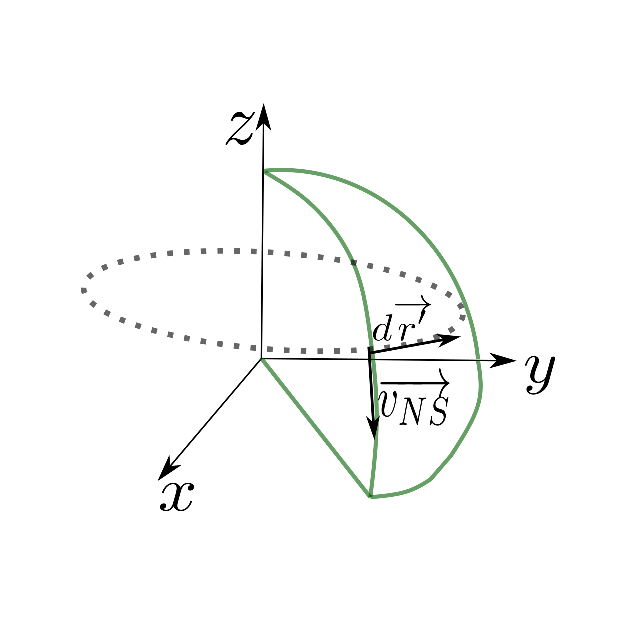
\includegraphics[width=5cm]{Coriolis_Force.eps}
 % \caption{北半球流线偏转示意图}\label{fig:71NorthStreamLine}
% \end{figure}

% 如图\ref{fig:71NorthStreamLine}所示,考虑一不与纬线平行的流线,其相对地球坐标系的涡量变化为(假设为正压流体):
% \begin{equation}
% \frac{D \Gamma'}{D t}=\oint_l -\v{a} \cdot d\v{r'}
% \end{equation}
% 对于转动坐标系中的加速度,有
% \begin{equation}\label{eq:71accelerate}
% \v{a}=\v{\omega}\times(\v{\omega}\times\v{R'})+2\v{\omega}\times\v{v'}
% \end{equation}
% 第一项为向心加速度,与$\v{r'}$垂直,对于第二项,只有在南北向的相对速度分量(球坐标系中为$\v{e_{\theta}}$方向)起作用,
% 因此$(\v{\omega}\times\v{v_{NS}})\cdot d\v{r'} =\v{\omega}\cdot(\v{v_{NS}}\times d\v{r'})$
% Physical Meaning Of Velocity Circuit?
% \begin{equation}
% \end{equation}

Lamb 型方程:考虑对理想气体,由欧拉方程\eqref{eq:62EulerEq}式和\eqref{eq:71vvw}式得到
\begin{equation}\label{eq:71Lamb}
 \frac{\partial \v{v}}{\partial t}+\nabla(\frac{1}{2}|\v{v}|^2)-\v{v}\times \v{\Omega}=\v{f}-\frac{1}{\rho}\nabla\cdot p
\end{equation}
其中$\v{v}\times \Omega$被称为Lamb矢量,若考虑质量力有势的正压定常流体,上式沿流线或涡线积分即可得到Bernoulli守恒方程:
\begin{equation}
\int_l \v{s}\cdot (\nabla(\frac{1}{2}|\v{v}|^2)-\v{v}\times \v{\Omega})ds=\int_l \v{s}\cdot (-\nabla\Pi-\nabla \mathbb{P})ds
\end{equation}
注意到$\v{s}$与$\v{v}$或$\v{\Omega}$平行,因此$\v{s}\cdot(\v{v}\times \v{\Omega})=0$,于是得到
\begin{equation}\label{eq:71LambBernoulli}
\frac{1}{2}v^2+\mathbb{P}+\Pi=C
\end{equation}
针对\eqref{eq:71Lamb}式,如考虑用常比热完全气体的等熵过程($\frac{p}{\rho^{\gamma}}=c$)代替正压的条件,则压力势项可改写为
\begin{align*}
\mathbb{P}=&\int \frac{dp}{\rho}\\
=& \int c\frac{d\rho^{\gamma}}{\rho}\\
=& \int c \gamma d \rho^{\gamma-2} d\rho\\
=& \int c \frac{\gamma}{\gamma-1} \rho^{\gamma-1}\\
=& \frac{\gamma}{\gamma-1}\frac{p}{\rho}
\end{align*}
因此对常比热完全气体的等熵过程,Bernoulli方程为
\begin{equation}
\frac{1}{2}v^2+\frac{\gamma}{\gamma-1}\frac{p}{\rho}+\Pi=C
\end{equation}
同理可推出对完全气体的等温过程
\begin{equation}
\frac{1}{2}v^2+RT\ln p+\Pi=C
\end{equation}
下面考虑流体相对等转速坐标系$O'x'y'$下的Bernoulli方程,转动坐标系相对静止坐标系的关系如下图所示:
\begin{figure}[!ht]
 \centering
 %LaTeX with PSTricks extensions
%%Creator: inkscape 0.92.2
%%Please note this file requires PSTricks extensions
%\documentclass{article}
%\pagestyle{empty}
%\usepackage{tikz}
%\begin{document}
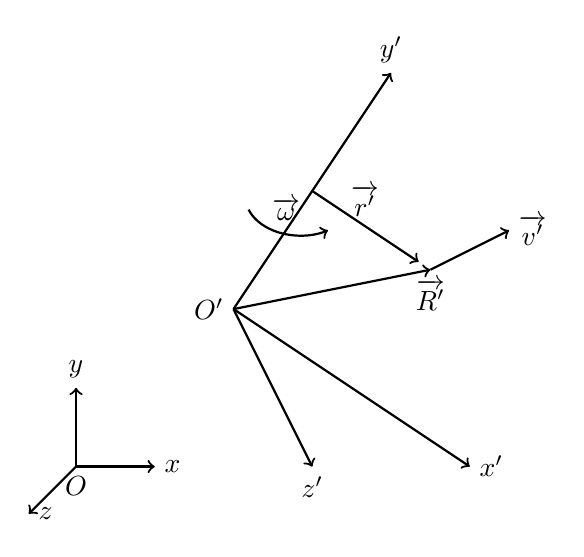
\begin{tikzpicture}
%reference coordinate 
  \draw[thick,->] (0,0) -- (1,0);
  \draw[thick,->] (0,0) -- (0,1);
  \draw[thick,->] (0,0) -- (-0.6,-0.6);  
  \draw (0,0) node[anchor=north] {$O$};  
  \draw (1,0) node[anchor=west] {$x$};      
  \draw (0,1) node[anchor=south] {$y$};      
  \draw (-0.6,-0.6) node[anchor=west] {$z$};      
  %rotational coordinate
  \draw[thick,->] (2,2) -- (5,0);
  \draw[thick,->] (2,2) -- (4,5);    
  \draw[thick,->] (2,2) -- (3,0);      
  \draw (2,2) node[anchor=east] {$O'$};  
  \draw (5,0) node[anchor=west] {$x'$};      
  \draw (4,5) node[anchor=south] {$y'$};      
  \draw (3,0) node[anchor=north] {$z'$};        
%point interested
  \draw[thick,->] (2,2) -- (4.5,2.5);%R'
  \draw[thick,->] (4.5,2.5) -- (5.5,3);%v'  
  \draw (4.5,2.5) node[anchor=north] {$\v{R'}$};    
  \draw (5.5,3) node[anchor=west] {$\v{v'}$};      
  \draw[thick,->] (3,3.5) -- (4.35,2.6);%r'
  \draw (3.67,3.05) node[anchor=south] {$\v{r'}$};
  \draw (2.67,3) node[anchor=south] {$\v{\omega}$};  
  \draw[thick,<-] (3.2,3) arc [start angle=300, end angle=200, x radius=0.7, y radius=0.5];
  \end{tikzpicture}
%\end{document}

 \caption{等转速坐标系下的Bernoulli方程推导示意}\label{fig:71rotationalCoordinateBernoulli}
\end{figure}
这里,我们去掉正压流体的假设,而附加绝热条件,于是\eqref{eq:62Enthalpy}式焓的随体导数可简化为:
\begin{align*}
\frac{D i}{D t} = &\frac{1}{\rho} \frac{D p}{D t}\\
\Rightarrow  \v{v}\cdot \nabla i =& \frac{1}{\rho} \v{v}\cdot \nabla p
\end{align*}
最后一式用到了定常流的条件,由于$\v{v}$的任意性,所以$\nabla i = \frac{\nabla p}{\rho}$,即
$\frac{\nabla p}{\rho}$有势函数$i$。

从\eqref{eq:71Lamb}式出发,由于是在转动坐标系中,我们对$\v{f}$有加速加项的修正,即以$\v{f}-\v{a}$
代替\eqref{eq:71Lamb}式中的$\v{f}$。$\v{a}$的表达式由\eqref{eq:71accelerate}式给出
\begin{equation}\label{eq:71accelerate}
\v{a}=\v{\omega}\times(\v{\omega}\times\v{R'})+2\v{\omega}\times\v{v'}
\end{equation}

注意到$\v{a}$的第二项$\v{v'}$含$\v{v'}$,如沿相对流线积分,同样由$\v{s'}$与$\v{v'}$平行的性质得其积分为零,因此,只需考虑
$\v{a}$的第一项
\begin{equation}\label{eq:71MiddleResultOmega}
\v{\omega}\times(\v{\omega}\times\v{R'}) = (\v{\omega}\cdot \v{R'})\v{\omega}-(\v{\omega}\cdot \v{\omega})\v{R'}
\end{equation}
我们这里设$\v{\omega}$沿$y'$轴,即$\v{\omega}=\omega \v{e_{y'}}$,
考虑$(\v{\omega}\cdot \v{\omega})\v{R'}$在$\v{e_{y'}}$方向的投影为$\omega^2(\v{R'}\cdot \v{e_{y'}})$,而
$(\v{\omega}\cdot \v{R'})\v{\omega}=\omega^2(\v{R'}\cdot \v{e_{y'}})\v{e_{y'}}$,因此\eqref{eq:71MiddleResultOmega}式可化简为
$(\v{\omega}\cdot \v{\omega})\v{R'}$在$O'x'z'$平面上的投影长度的相反数:
%\begin{align*}
%\end{align*}
\begin{equation}
\v{\omega}\times(\v{\omega}\times\v{R'})=-\omega^2 \v{r'}
\end{equation}
其中$\v{r'}$为$\v{R'}$在$Ox'z'$平面上的投影向量,并假设转动角速度$\omega$为常数,则
\begin{equation}
\v{\omega}\times(\v{\omega}\times\v{R'})=-\nabla' (\frac{1}{2}\omega^2 r'^2)
\end{equation}
这里$\nabla'$表示相对转运坐标系的梯度算子,所以$\v{a}$项在沿相对流线积分得到$\frac{1}{2}\omega^2 r'^2$。
综合上面的结果,我们得到等转速坐标系下的Bernoulli方程为:
\begin{equation}
\frac{1}{2}v'^2+\Pi+i-\frac{1}{2}\omega^2 r'^2 = c
\end{equation}
\begin{equation}
\end{equation}
\begin{equation}
\end{equation}

\begin{thebibliography}{99}
\bibitem{mixedProduct} \href{https://en.wikipedia.org/wiki/Triple_product}{https://en.wikipedia.org/wiki/Triple\_product}
\bibitem{velocityGradient}\href{http://www.continuummechanics.org/velocitygradient.html}{http://www.continuummechanics.org/velocitygradient.html}
\bibitem{angularVelocityTensor}\href{https://en.wikipedia.org/wiki/Angular_velocity#Angular_velocity_tensor}{https://en.wikipedia.org/wiki/Angular\_velocity\#Angular\_velocity\_tensor}
\bibitem{CylindricalCoordinates}\href{https://en.wikipedia.org/wiki/Divergence#Cylindrical_coordinates}{https://en.wikipedia.org/wiki/Divergence\#Cylindrical\_coordinates}
\bibitem{CurlFormular}\href{https://en.wikipedia.org/wiki/Curl_(mathematics)}{https://en.wikipedia.org/wiki/Curl\_(mathematics)}
\bibitem{FundamentalSolution}\href{https://en.wikipedia.org/wiki/Fundamental_solution}{https://en.wikipedia.org/wiki/Fundamental\_solution}
\bibitem{GreenFunction}\href{https://en.wikipedia.org/wiki/Green\%27s_function#Green.27s_functions_for_the_Laplacian}{https://en.wikipedia.org/wiki/Green\%27s\_function\#Green.27s\_functions\_for\_the\_Laplacian}
\bibitem{Del}\href{https://en.wikipedia.org/wiki/Del_in_cylindrical_and_spherical_coordinates}{https://en.wikipedia.org/wiki/Del\_in\_cylindrical\_and\_spherical\_coordinates}
\bibitem{CEEquation}\href{https://en.wikipedia.org/wiki/Cauchy\%E2\%80\%93Euler_equation}{https://en.wikipedia.org/wiki/Cauchy\%E2\%80\%93Euler\_equation}
\end{thebibliography}
\end{document}